\documentclass[handout]{beamer}

\mode<presentation>
{
  \usetheme{default}      % or try Darmstadt, Madrid, Warsaw, ...
  \usecolortheme{default} % or try albatross, beaver, crane, ...
  \usefonttheme{serif}  % or try serif, structurebold, ...
  \setbeamertemplate{navigation symbols}{}
  \setbeamertemplate{caption}[numbered]
}

\newcommand{\Prob}{\text{Prob}}
\newcommand{\bx}{\mathbf{x}}
\newcommand{\bphi}{\pmb{\phi}}
\newcommand{\btheta}{\pmb{\theta}}
\newcommand{\Count}{\text{count}}
\newcommand{\given}{\, | \,}
\newcommand{\diag}{\text{diag}}
\DeclareMathOperator*{\argmax}{arg\,max}

%\usepackage{pgfpages}
%\pgfpagesuselayout{4 on 1}[a4paper,border shrink=5mm]

\title{A Brief on Natural Language Processing}
\author{Luis Berlioz}
\begin{document}
\maketitle

%%%%FRAME
\begin{frame}{Natural Language Processing (NLP)}
    Using Machine Learning techniques with Human Language.
    \begin{itemize}
            \item AKA Computational Linguistics.
            \item Goes from a continuous medium (airwaves) to a discrete (text).
        \item Traditionally, speech processing is done by electrical engineers and NLP by C.S. people.
            \item Really complex, consider the following headline:
                \begin{itemize}
                    \item \textit{``Scientists study whales from space.''}
                \end{itemize}
    \item No A.I. program could be said to be complete without the ability to communicate in words.
        \item Important role in Search and Text Mining.
    \end{itemize}
     
\end{frame}

%%%%FRAME
\begin{frame}{Summary}
    \begin{itemize}
            \item Example: Paragraph Classification
            \item Classification Method: Na\"ive Bayes
            \item Word embeddings
            \item Example GloVe on the ArXiv 
    \end{itemize}
\end{frame}
%%%%FRAME
\begin{frame}{Common Terminology for Classification Problemks}
    \begin{exampleblock}{Vocabulary}
        The set $V = \{w_1,w_2,\ldots, w_V\}$ of all the \textit{words} or \textit{tokens}.
    \end{exampleblock}
        \begin{itemize}
            \item \textbf{Common Crawl (uncased)} 42B tokens, 1.9M vocab.
            \item \textbf{Common Crawl (cased)} 840B tokens, 2.2M vocab.
            \item \textbf{Twitter} 2B tweets, 27B tokens, 1.2M vocab
            \item \textbf{Wikipedia 2014 + Gigaword 5} 6B tokens 400K vocab
            \item \textbf{arXiv.org} 1,000,295 vocab.arxmliv.txt
        \end{itemize}

        \begin{exampleblock}{Labels or Classes}
            The set of labels $\{y^{(1)},y^{(2)},\ldots, y^{(n)}\}$\\
            In the example these were: \textbf{Definitions, Examples, Propositions, etc}.
        \end{exampleblock}


\end{frame}

\begin{frame}{Bag of Words Model}
    Represent a document, email, tweet as a vector $\bx=(x_1,\ldots, x_V)$
    \begin{columns}[T]
        \begin{column}{0.6\textwidth}
            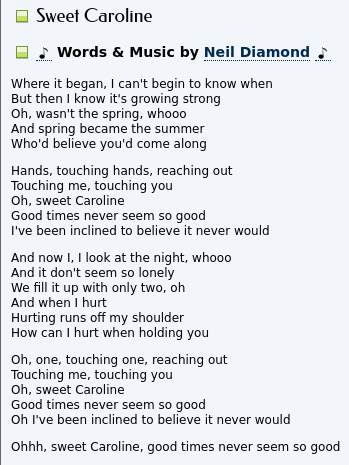
\includegraphics[width=0.9\textwidth]{sweet_caroline_lyrics.png}
        \end{column}
        \begin{column}{0.4\textwidth}
            \begin{tabular}{|c|l|c|}
                \hline
                \hline
                $V$ & TOK& Freq. \\
                \hline
                \hline
                23 & oh&6\\
                \hline
                4500 & touching&6\\
                \hline
                10 & good&6\\
                \hline
                80 & never&5\\
                \hline
                50 & seem&4\\
                \hline
                38 & believe&3\\
                \hline
                99 & sweet&3\\
                \hline
                43 & caroline&3\\
                \hline
                30 & time&3\\
                \hline
                90 &know&2\\
                \hline
                54& spring&2\\
                \hline
                897& whooo&2\\
                \hline
                230 & hand&2\\
                \hline
                654 & reaching&2\\
                \hline
            \end{tabular}
        \end{column}
    \end{columns}
\end{frame}

\begin{frame}{Na\"ive Bayes}
    Suppose we have a long list of $N$ labeled documents $$\{(\bx^{(i)},y^{(i)}) :\ i = 1,\ldots, N \}$$
        And $\bx^{(i)}\given y^{(i)} $ has a Multinomial distribution with parameters $\bphi = (\phi_1,\ldots, \phi_V)$ 
        $$\Prob(\bx\given y;\bphi) = \frac{(\sum_{j=1}^V x_j)!}{x_1!\cdots x_V!}\  \prod_{j=1}^V \phi_j^{x_j}$$

        We are interested in:
        $$\Prob(y\given \bx) = \frac{\Prob(y)\  \Prob(\bx \given y; \bphi)}{\Prob(\bx)}\propto \Prob(\bx, y,\bphi)$$
        Since:
        $$\Prob(\bx,y; \bphi) = \Prob(y) \ \Prob(\bx \given y; \bphi)$$

\end{frame}


%%%%FRAME
\begin{frame}{Na\"ive Bayes (Prediction)}
     We choose the label that maximizes the joint probability:
     $$\hat y = \argmax_y\left\{ \Prob(\bx, y: \bphi)\right \}$$
     Equivalently:
     $$\hat y = \argmax_y\left\{ \log \Prob(\bx\given y: \bphi) + \log\Prob(y)\right\}$$
     {\color{green}Reminder:} $\displaystyle \Prob(\bx\given y;\bphi) = B(\bx) \prod_{j=1}^V \phi_j^{x_j}$\\
     Substituting inside the log:
     $$= \log B(\bx) + \btheta\cdot f(\bx, y)$$
    Where $\btheta = [\log \phi_{y,1}, \log \phi_{b,2} ,\ldots , \log \phi_{y,V}; \log \hat y]$
\end{frame}


%%%%FRAME
\begin{frame}{Na\"ive Bayes (Estimation)}
    We use the labels to find $\bphi$ as follows:
    \begin{align*}
     \hat\bphi &= \argmax_{\bphi} \left\{ \Prob(\bx, y; \bphi)\right \}\\
      &= \argmax_{\bphi} \prod_{i=1}^N \Prob(\bx^{(i)}, y^{(i)}; \bphi)\\
     &= \argmax_{\bphi} \sum_{i=1}^N \log \Prob(\bx^{(i)}, y^{(i)}; \bphi)\\
    \end{align*}
    The parameters are given by:
    $$\phi_{y,j} = \frac{\Count(y,j)}{\sum_{j'=1}^{V}\Count(y,j') + \alpha}$$
    \begin{itemize}
        \item $\Count(y,j)$ is the number word $j$-s in $y$ labeled documents. 
        \item Where $\alpha>0$ because no parameter can be zero.
    \end{itemize}
\end{frame}

%%%%FRAME
\begin{frame}{More about Classification}
    Other powerful methods for classification include:
    \begin{itemize}
            \item Random Forests
            \item Perceptron and Logistic Regression
    \end{itemize}
    How can we use Neural Networks for NLP?
    \begin{itemize}
            \item Reduce the dimension, $V$ is too big for a NN.
    \end{itemize}
    \begin{figure}[c]
        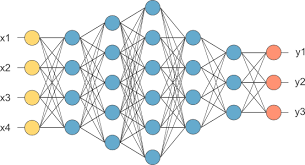
\includegraphics[width=0.6\textwidth]{nn.png}
    \end{figure}
\end{frame}

\begin{frame}{Similarity based representations}
    \begin{block}{One-hot Representation}
        It has 1 in index of the word and 0 elsewhere
        $$\text{word} \mapsto [0,0,0,\ldots,0,1,0,\ldots,0,0,0,0]$$
        But we would like:
        \begin{itemize}
            \item Smaller dimension.
            \item Similar words are close by.
        \end{itemize}
    \end{block}
    ``You shall know a word by the company it keeps''\\[5mm]
    \hspace*\fill{\small John R. Firth}

    We will talk about three methods
    \begin{itemize}
            \item SVD to co-ocurrence matrix
            \item Skip-Gram Model
            \item Global Vectors (GloVe)
    \end{itemize}

\end{frame}

%%%%FRAME
\begin{frame}{Co-ocurrence Matrix}
    \begin{figure}[c]
    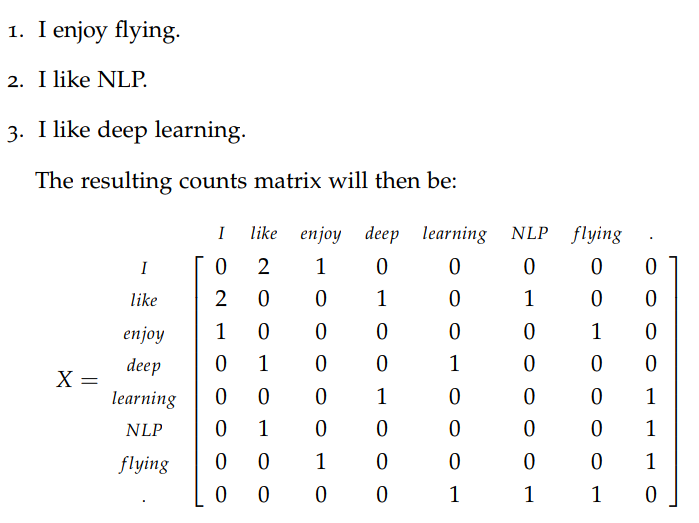
\includegraphics[width=0.75\textwidth]{coocurrence_matrix.png}
    \end{figure}
    \begin{itemize}
        \item Observe that \textit{like} and \textit{enjoy} are NOT orthogonal.
    \end{itemize}
\end{frame}

%%%%FRAME
\begin{frame}{Co-ocurrence Matrix}
Let $X = U\Sigma W^T$ be the SVD of $X$
    $$ U = [u_1 \given u_2\given \cdots ]\quad \Sigma = \diag(\sigma_1,\ldots, \sigma_V)\quad W = \begin{bmatrix}-& w_1&- \\-& w_2&- \\ &\vdots& \end{bmatrix}$$
        Approximate $X$ by taking $k<V$ singular values:
        $$\hat X = \sum_{t=1}^k \sigma_t\, u_k\, W_k^T\approx X$$
        \begin{itemize}
                \item Above, $W_k^T$ are the columns of $W$.
        \item The one-hot vector are embedded in $k$-dimensional space as the vectors $\bar w_k^T$.
        \end{itemize}
\end{frame}

\begin{frame}{Similarity based representations}
    If $w_t$ is the word we care about and $w_{t +j}$ denotes the words to the left-right:
    $$\Prob(w_{t+j}\given w_t)$$
    \begin{itemize}
        \item $\Prob(w_{t-1}=\text{cauchy} \given w_t=\text{sequence})$ should be high.
        \item $\Prob(w_{t+1}=\text{infinite} \given w_t=\text{finite})$ should be very low.
    \end{itemize}
    \begin{figure}[c]
    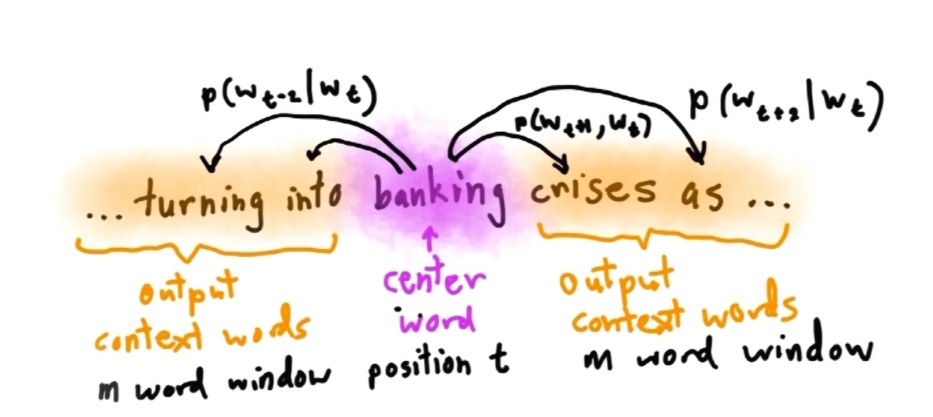
\includegraphics[width=0.7\textwidth]{skipgram.png}
    \end{figure}
\end{frame}

%%%%FRAME
\begin{frame}{Setup of Skip-Gram}
    Given a word $w_t$ we want to predict its \textit{context:} $$C_{w_t} = \{w_{t+j} :\ |j|\leq m \text{ and } j \neq 0\}$$
    $$\mathcal J(\btheta) = \prod_{t=1}^T\  \prod_{\substack{|j|\leq m\\ j\neq 0}} \Prob(w_{t+j}\given w_t; \btheta)$$
    $$J(\btheta) = \frac 1T \sum_{t=1}^T \sum_{\substack{|j|\leq m\\ j\neq 0}}\log \Prob(w_{t+j}\given w_t; \btheta)$$
    We want to find $\hat \btheta  = \argmax_{\btheta} J(\btheta)$.
\end{frame}

%%%%FRAME
\begin{frame}{Skip-Gram }
    We use two type of Parameters:
    \begin{itemize}
            \item $v_t$ for estimating $w_t$ as a center word.
            \item $u_{t-m}, \ldots u_{t-1}, u_{t+1}, \ldots , u_{t+m}$ for $w_t$ as a context word.
            \item $\btheta = (U,W)$ are matrices, $v_t = W\, x$ ($x$ is the one-hot representation of $w_t$.)
    \end{itemize}
    $$\prod_{\substack{|j|\leq m\\ j\neq 0}}\Prob(w_{t+j}\given w_t; \btheta) =    \prod_{\substack{|j|\leq m\\ j\neq 0} } \Prob(u_{t+j} \given v_t)$$
    We estimate this last probability as a softmax:
    $$\Prob(u_{t+j}\given v_t) = \frac{\exp(u^T_{t+j}v_t)}{ \sum_{n=1}^V \exp(u_n^T v_n)}$$
\end{frame}

%%%%FRAME
\begin{frame} 
    Remember:
    $$J(\btheta) = \frac 1T \sum_{t=1}^T \sum_{\substack{|j|\leq m\\ j\neq 0}}\log \Prob(w_{t+j}\given w_t; \btheta)$$
    And:
    $$\Prob(u_{t+j}\given v_t) = \frac{\exp(u^T_{t+j}v_t)}{ \sum_{n=1}^V \exp(u_n^T v_n)}$$
     Putting everything together:
     $$ J(U,W) = \sum_{\substack{|j|\leq m\\ j\neq 0}} u_{t+j}^Tv_t - 2m\log \sum_{n=1}^V \exp(u_n^T v_n)$$
\end{frame}
%%%%FRAME
\begin{frame}{GloVe Project}
    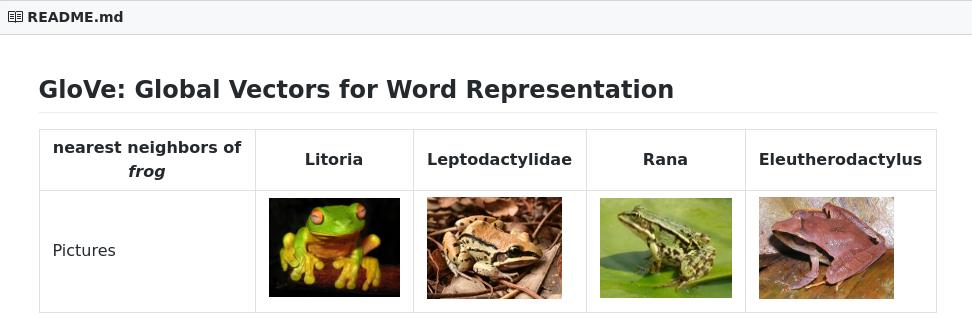
\includegraphics[width=\textwidth]{Glove_github_small.png}

\begin{figure}
   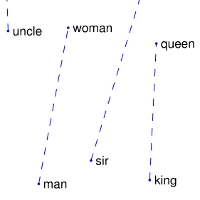
\includegraphics[width=0.29\textwidth]{man_woman_small.jpg}
   \hfill
   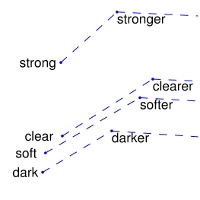
\includegraphics[width=0.29\textwidth]{comparative_superlative_small.jpg}
   \hfill
   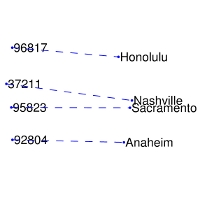
\includegraphics[width=0.29\textwidth]{city_zip_small.jpg}
\end{figure}

\end{frame}

%%%%FRAME
\begin{frame}{Advantages of Similarity based Representation}

    \begin{itemize}
        \item Better classification because similar concepts cluster together.
        \item Sentiment Analysis can actually worsen with word embeddings.
        \item Smaller dimension work better for input to NN.
    \end{itemize}
\end{frame}

%%%%FRAME
\begin{frame}{The Formal Abstracts Project}
    \begin{block}{Formal Abstracts}
        A \textit{formal abstract}, or fabstract for short, is a formalization of the main results (constructions, definitions, proofs, conjectures) of a piece of informal mathematics, such as a research paper.
    \end{block}
    Big Goals, tons of applications for ML and NLP:
    \begin{itemize}
            \item Translate Natural language into a computer checkable format.
            \item Detecting errors in the mathematical literature, and intelligent mathematical search tools.
    \end{itemize}
\begin{figure}
   
\includegraphics[width=0.45\textwidth]{lean_website.png}
   \hfill
   
\includegraphics[width=0.45\textwidth]{fabstract_log.jpeg}
\end{figure}
\end{frame}
\end{document}
